% http://www.ctan.org/tex-archive/macros/latex/contrib/beamer/examples
% http://latex.artikel-namsu.de/english/beamer-examples.html

%\documentclass{beamer}
\documentclass[usenames,dvipsnames,12pt,compress]{beamer}
\setbeamertemplate{navigation symbols}{}
\usepackage[utf8]{inputenc}
\usepackage{amsmath}
\usepackage{amssymb}
\usepackage{bm}
\usepackage{fancybox, graphicx}
\usepackage{listings}
\usepackage{tikz} % Diagrams
\usetikzlibrary{positioning}
\usepackage{color}
\usepackage{textcomp} % See https://tex.stackexchange.com/questions/145416/how-to-have-straight-single-quotes-in-lstlistings
%\usepackage[font=small,labelfont=bf]{caption} % Required for specifying captions to tables and figures. From https://tex.stackexchange.com/questions/238636
\usepackage[absolute,overlay]{textpos}
\usepackage[T1,T2A]{fontenc} % See https://tex.stackexchange.com/questions/135118
\usepackage[russian,english]{babel}
\usepackage{url}


\lstset{language=bash,upquote=true} % Format listings as appropriate for bash. Inexplicably we get problems if the language is set as part of the \begin{lstlisting} command.

% https://tex.stackexchange.com/questions/36030/how-to-make-a-single-word-look-as-some-code
\definecolor{light-gray}{gray}{0.95}
\newcommand{\code}[1]{\colorbox{light-gray}{\texttt{#1}}}

\newcommand{\mentiurl}[0]{{\url{www.menti.com}}}
\newcommand{\menticode}[0]{{14 11 05 9}}
\newcommand{\mentiinvitation}[0]{Go to \mentiurl{} (code \menticode{}) and choose:\\}
\newcommand{\correctanswer}[1]{\textcolor{blue}{{#1} \checkmark}}

% Parameters: file name, graphics options (e.g. `scale=0.3'), whom to credit, x pos for credit, y pos for credit.
\newcommand{\imageandcredit}[5]{
  {
    \begin{tikzpicture}
      \draw (-4, 0) node[inner sep=0] {\includegraphics[{#2}]{{#1}}};
      \draw ({#4},{#5}) node[white,fill=black,font=\tiny] {Credit: {#3}};
    \end{tikzpicture}
  }
}

% Parameters: file name, graphics options (e.g. `scale=0.3'), background colour, whom to credit, x pos for credit, y pos for credit.
\newcommand{\framewithimageandcredit}[6]{
{
  \setbeamercolor{background canvas}{bg={#3}}
  \begin{frame}{}
    \begin{center}
      \imageandcredit{#1}{#2}{#4}{#5}{#6}
    \end{center}
  \end{frame}
 }
}


%Parameters: Item text, file name, graphics options, whom to credit, x pos for credit, y pos for credit.
\newcommand{\itemandimageandcredit}[6]{
  \begin{columns}
  \column{0.04\linewidth}
  \column{0.41\linewidth}
  \item{#1}
  \column{0.55\linewidth}
  \imageandcredit{#2}{#3}{#4}{#5}{#6}
  \end{columns}
}


%\usetheme{boxes}
%\usecolortheme{beaver}


\title{The Constantly Changing Hubble Constant}
\author{Lorne Whiteway \\ lorne.whiteway@star.ucl.ac.uk}
\institute{Astrophysics Group \\ Department of Physics and Astronomy \\ University College London}
\date{Presentation to the Mid-Kent Astronomical Society \\ 12 November 2021 \\ You are invited to go to \alert{\mentiurl{}} and enter code \menticode{}.}

\begin{document}

\frame{\titlepage}


\begin{frame}{The Universe is expanding!}
  \begin{itemize}
  \item{But what does this actually mean?}
  \item{How do we know it is expanding?}
  \item{Why is it expanding?}
  \item{How fast is it expanding? How do we measure this?}
  \item{Is the expansion rate changing?}
  \end{itemize}
\end{frame}


\begin{frame}{How do we know?}
  \begin{columns}
    \column{0.4\linewidth}
    \begin{itemize}
    \item{Everywhere we look, distant galaxies are receding; more distant galaxies are receding faster.}
    \item{So either we are at the centre of a cosmic conspiracy, or all the space between all the galaxies is expanding.}
    \end{itemize}
    \column{0.6\linewidth}
    \centering
    \imageandcredit{720px-Hubble_ultra_deep_field_high_rez_edit1.jpg}{height=7cm}{NASA Ultra Deep Field}{-5.7}{-3.2}
  \end{columns}
\end{frame}


\begin{frame}{Is the solar system expanding? Are \textit{we} expanding?}
    \mentiinvitation{}
    \begin{enumerate}
      \item{Yes, a lot}
      \item{Yes, but only a tiny amount}
      \item{No}
    \end{enumerate}
\end{frame}


\begin{frame}{Is the solar system expanding? Are \textit{we} expanding?}
    \mentiinvitation{}
    \begin{enumerate}
      \item{Yes, a lot}
      \item{Yes, but only a tiny amount}
      \item{\correctanswer{No}}
    \end{enumerate}
\end{frame}


\begin{frame}{Is the solar system expanding? Are \textit{we} expanding?}
    \begin{itemize}
      \item{Other forces - molecular forces between the molecules in your body, and gravitational forces between the Sun and the planets - are far more than strong enough to overcome the effect of cosmic expansion.}
      \bigskip
      \itemandimageandcredit{Gravity is even strong enough to keep the Andromeda Galaxy from receding from us.}{Andromeda_Galaxy_560mm_FL.jpg}{height=2.5cm}{David Dayag}{-3.25}{-1.48}
      \bigskip
	\item{It's only the furthest objects - where gravity becomes negligible - that recede.}
    \end{itemize}
\end{frame}


\begin{frame}{What does \textit{recession velocity} actually mean?}
  \begin{itemize}
  \item{We say `distant galaxies are moving away from us'. This is informal language.}
  \item{They aren't really moving, they just appear to be - because the intervening space is expanding.}
  \bigskip
  \item{Sometimes this distinction is important - for example, the recession velocity can exceed the speed of light.}
  \end{itemize}
\end{frame}


\begin{frame}{Which `Ed' first had the idea that the Universe is expanding?}
    \mentiinvitation{}
    \begin{enumerate}
      \item{Edmond Halley}
      \item{Edwin Hubble}
      \item{Edgar Allan Poe}
    \end{enumerate}
\end{frame}


\begin{frame}{Which `Ed' first had the idea that the Universe is expanding?}
    \mentiinvitation{}
    \begin{enumerate}
      \item{Edmond Halley}
      \item{Edwin Hubble}
      \item{\correctanswer{Edgar Allan Poe}}
    \end{enumerate}
\end{frame}


\begin{frame}{History}
  \begin{itemize}
  \itemandimageandcredit{In 1848 Edgar Allan Poe published \textit{Eureka}, which included a description of expanding space.}{512px-Edgar_Allan_Poe,_circa_1849,_restored,_squared_off.jpg}{height=4cm}{Public domain}{-4}{-2.2}
  \item{Expansion is not obvious without large telescopes and so isn't usually part of pre-modern cosmologies. Full understanding only came in the 20th century.}
  \end{itemize}
\end{frame}


\begin{frame}{So how fast is the expansion?}
  \begin{itemize}
  \item{For every additional distance of one megaparsec, there's an additional recession velocity of about 70 kilometers per second.}
  \item{So the expansion speed is about 70 kilometers per second per megaparsec.}
  \bigskip
  \item{One megaparsec is about three million light years. It's the typical distance between galaxies.}
  \item{70 kilometers per second is about 150,000 miles per hour.}
  \end{itemize}
\end{frame}


\begin{frame}{So how fast is the expansion?}
    \begin{tikzpicture}
    \node at (4,1) {Start with a distance:};
    \draw [very thick] (0,0)--(10,0);
    \pause
    \node at (4,-2) {13.5 million years later it will be 1\% longer:};
    \draw [very thick] (0,-3)--(10.1,-3);
    \pause
    \node at (4,-5) {Continental drift is about six times faster...};
    \end{tikzpicture}
\end{frame}


\begin{frame}{$H_0$}
  \begin{itemize}
  \item{The current expansion rate is called the \textit{Hubble constant} or \textit{Hubble parameter} and is denoted `$H_0$'.}
  \bigskip
  \itemandimageandcredit{The `$H$' commemorates Edwin Hubble (1889-1953), who was one of the first to measure it.}{Studio_portrait_photograph_of_Edwin_Powell_Hubble.jpg}{height=3cm}{Johan Hagemeyer}{-4}{-1.3}
  \bigskip
  \item{The `$0$' refers to today. The expansion rate was different in the distant past.}
  \end{itemize}
\end{frame}
 
 
\begin{frame}{Why does the Universe expand?}
  \begin{itemize}
  \item{Science is not so good with `why?' questions...}
  \bigskip
  \item{There's an \textit{initial condition}: the Universe started expanding at the Big Bang.}
  \bigskip
  \item{The later behaviour of the expansion (does it slow down? speed up?) then depends, essentially via gravity, on \textit{what's in the Universe}.}
  \end{itemize}
\end{frame}
  
  
\begin{frame}{Why does gravity play a role?}
  \begin{itemize}
  \itemandimageandcredit{\textit{General relativity}, our modern theory of gravity, is due to Einstein (1916).}{08608_einstein_1916.jpg}{height=6cm}{Paul Ehrenfest}{-5.03}{-3.2}
  \end{itemize}
\end{frame}


\begin{frame}{Why does gravity play a role?}
  \begin{itemize}
  \item{Remember \textit{mass} and \textit{energy} are the same ($E=mc^2$).}
  \bigskip
  \itemandimageandcredit{Mass/Energy \textit{bends} spacetime, essentially changing distances and angles.}{800px-Spacetime_lattice_analogy.svg.png}{height=2cm}{Mysid}{-4}{-1.3}
  \end{itemize}
\end{frame}


\begin{frame}{Why does gravity play a role?}
  \begin{itemize}
  \item{This `changing of distances and angles' works locally; the distorted spacetime governs how objects move, and this leads e.g. to the apple falling from the tree.}
  \bigskip
  \pause
  \item{But it also works on the Universe as a whole - mass/energy can cause distances to change \textit{everywhere} in the Universe - and in particular can lead to increasing distances everywhere. This is the expansion that we see.}
  \end{itemize}
\end{frame}


\begin{frame}{Contents of Universe control expansion}
  \begin{itemize}
  \itemandimageandcredit{It was Alexander Friedmann (\begin{otherlanguage*}{russian}Алекс\'{а}ндр Алекс\'{а}ндрович Фр\'{и}дман\end{otherlanguage*}) (1888-1925) who first realised this (1922).}{Aleksandr_Fridman.png}{height=6cm}{Public domain}{-4}{-3.2}
  \end{itemize}
\end{frame}


\begin{frame}{What if we go backwards in time?}
  \begin{itemize}
  %https://upload.wikimedia.org/wikipedia/commons/thumb/5/51/Georges_Lema%C3%AEtre_1930s.jpg/512px-Georges_Lema%C3%AEtre_1930s.jpg
  \itemandimageandcredit{George Lama\^itre (1894-1966) realised that if the Universe was expanding then it must, at an earlier stage, have been very small; he thereby invented the idea of the `Big Bang'.}{512px-Georges_Lemaitre_1930s.jpg}{height=6cm}{Public domain}{-4}{-3.2}
  \end{itemize}
\end{frame}


\begin{frame}{How do we measure the expansion rate?}
  \begin{itemize}
  \item{In theory it's easy: find a distant galaxy, measure its recession velocity and its distance, and take the ratio.}
  \bigskip
  \item{Example: a galaxy is receding at 1600 kilometers per second and is 20 megaparsecs away; \linebreak \bigskip then $H_0$ is 80 kilometers per second per megaparsec.}
  \end{itemize}
\end{frame}


\begin{frame}{Can use \textit{redshift} to measure recession velocity}
  \begin{itemize}
  \item{Light from distant galaxies gets stretched by the expansion; this makes it turn redder.}
  \bigskip
  \itemandimageandcredit{It's fairly easy to measure the amount of red-shifting, as spectral lines are a convenient reference point. The redshift then immediately gives the velocity.}{256px-Redshift.svg.png}{height=4cm}{Georg Wiora}{-4}{-2}
  \end{itemize}
\end{frame}


\begin{frame}{V M Slipher}
  \begin{itemize}
  \itemandimageandcredit{The first redshifts for galaxies (known then as nebulae) were made in 1912 by Vesto Slipher (1875 - 1969) at the Lowell Observatory in Flagstaff, Arizona.}{V.M._Slipher.png}{height=7cm}{Lowell Archives}{-4}{-3}
  \end{itemize}
\end{frame}


\begin{frame}{Recession velocity for galaxy M77}
  \begin{block}{}
  From Slipher's 1917 `Lowell Observatory Bulletin 80':
  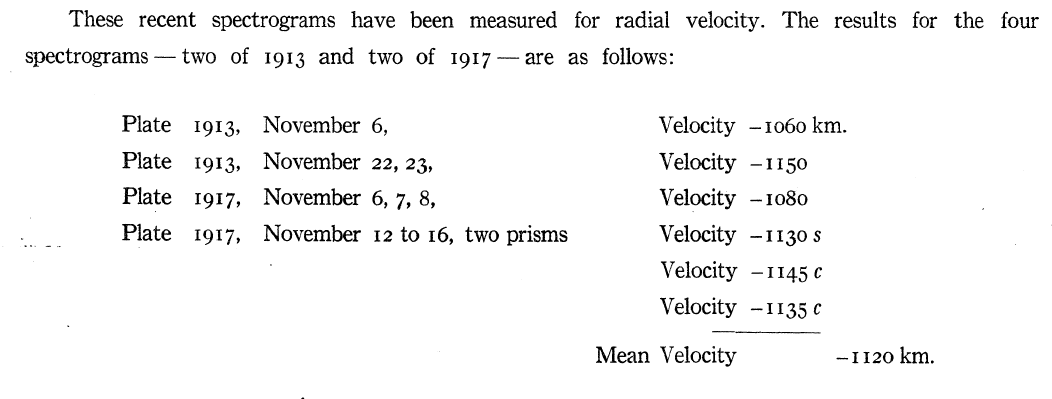
\includegraphics[height=4.2cm]{Slipher_1917_Lowell_Bulletin_80.png}
  \end{block}
  \begin{block}{}
  Modern value (from NASA/IPAC Extragalactic database):
  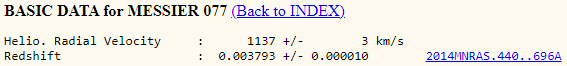
\includegraphics[height=1cm]{M77_Velocity.png}
  \end{block}
\end{frame}


\begin{frame}{Can use Cepheids to measure distance}
\begin{itemize}
\item{Cosmic distances can be estimated using variable stars called \textit{Cepheids}. We know how much light they produce (it's related to their period) - so they are \textit{standard candles}. Their observed brightness then tells us their distance.}
\itemandimageandcredit{The brightness/period relation was discovered by Henrietta Swan Leavitt (1868 - 1921) at Harvard.}{256px-Leavitt_aavso.jpg}{height=5cm}{Public Domain}{-4}{-3}
\end{itemize}
\end{frame}


\begin{frame}{How far away is that Cepheid?}
  \begin{block}{}
  $A$ and $B$ are two identical Cepheids; $A$ is 100 parsecs distant; $B$ is $4\%$ of the brightness of $A$. How far is $B$?
  \end{block}
  \begin{block}{}
    \mentiinvitation{}
    \begin{enumerate}
      \item{500 parsecs}
      \item{2500 parsecs}
      \item{4 parsecs}
    \end{enumerate}
  \end{block}
\end{frame}


\begin{frame}{How far away is that Cepheid?}
  \begin{block}{}
  $A$ and $B$ are two identical Cepheids; $A$ is 100 parsecs distant; $B$ is $4\%$ of the brightness of $A$. How far is $B$?
  \end{block}
  \begin{block}{}
    \mentiinvitation{}
    \begin{enumerate}
      \item{\correctanswer{500 parsecs}}
      \item{2500 parsecs}
      \item{4 parsecs}
    \end{enumerate}
  \end{block}
\end{frame}


\begin{frame}{Recession velocity vs distance relationship}
  \begin{itemize}
    \itemandimageandcredit{It was Lamaitre who first suggested a linear relationship between recession velocity and distance.}{MillikanLemaitreEinstein.jpg}{height=3cm}{Public domain}{-4}{-1.3}
    \itemandimageandcredit{Hubble then provided supporting evidence - he used the 100 inch telescope at Mt Wilson to spot Cepheids in a range of galaxies.}{edwin-hubble_custom-1ba7b4eff9a01a9787734122a061ed1926acd23c-s300-c85.jpg}{height=3cm}{Edwin Hubble Papers}{-4}{-1.3}
  \end{itemize}
\end{frame}


\begin{frame}{Hubble's plot - from 1929 PNAS paper}
%https://www.pnas.org/content/15/3/168/tab-figures-data
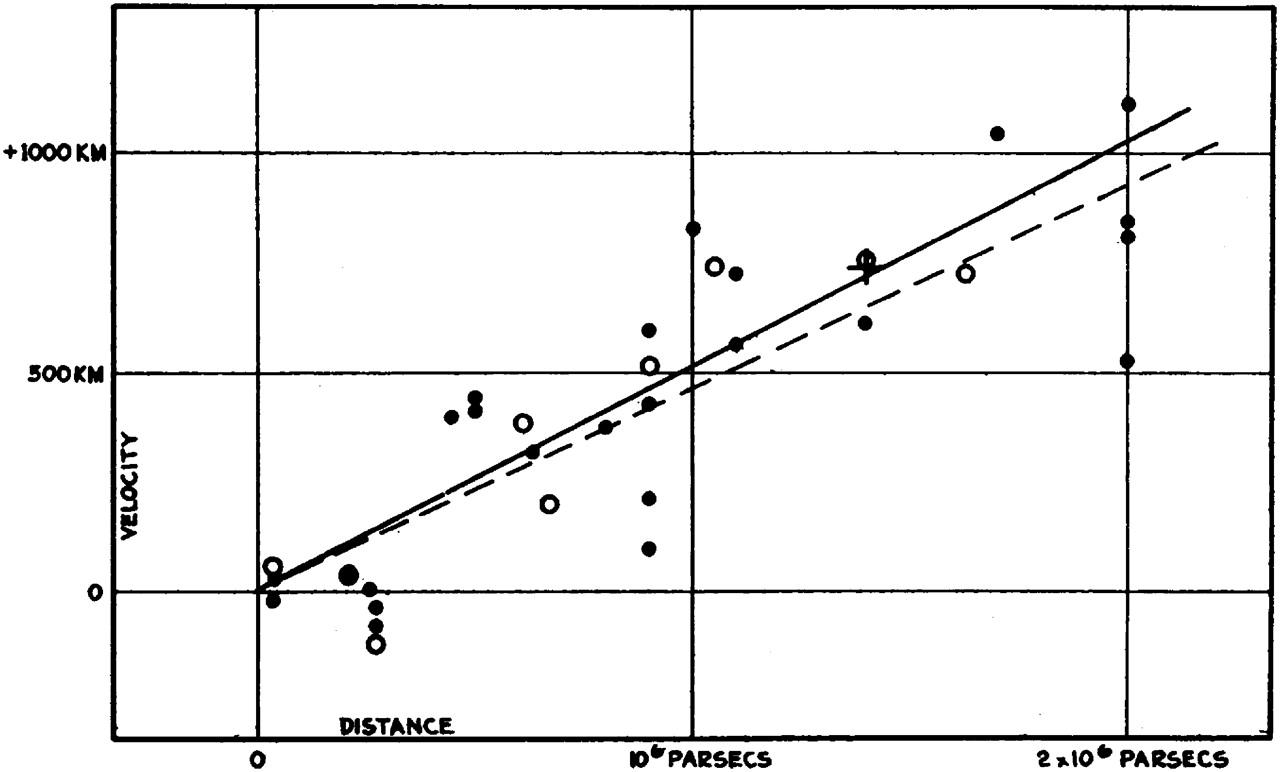
\includegraphics[height=6.8cm]{F2.large.jpg}
\end{frame}


\begin{frame}{What value for $H_0$ does this plot give?}
  \begin{block}{}
  %https://www.pnas.org/content/15/3/168/tab-figures-data
  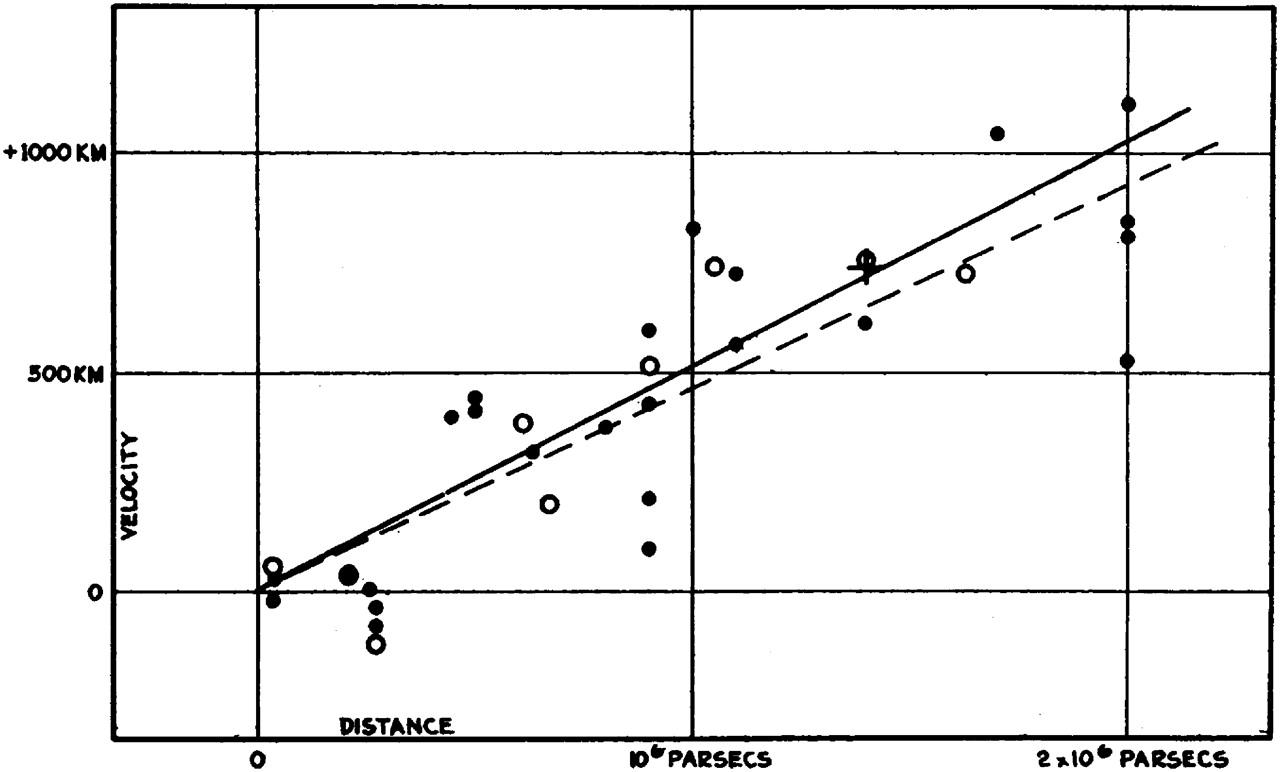
\includegraphics[height=4cm]{F2.large.jpg}
  \end{block}
  \begin{block}{}
    \mentiinvitation{}
    \begin{enumerate}
      \item{70 km per second per megaparsec}
      \item{100 km per second per megaparsec}
      \item{500 km per second per megaparsec}
    \end{enumerate}
  \end{block}
\end{frame}


\begin{frame}{What value for $H_0$ does this plot give?}
  \begin{block}{}
%https://www.pnas.org/content/15/3/168/tab-figures-data
  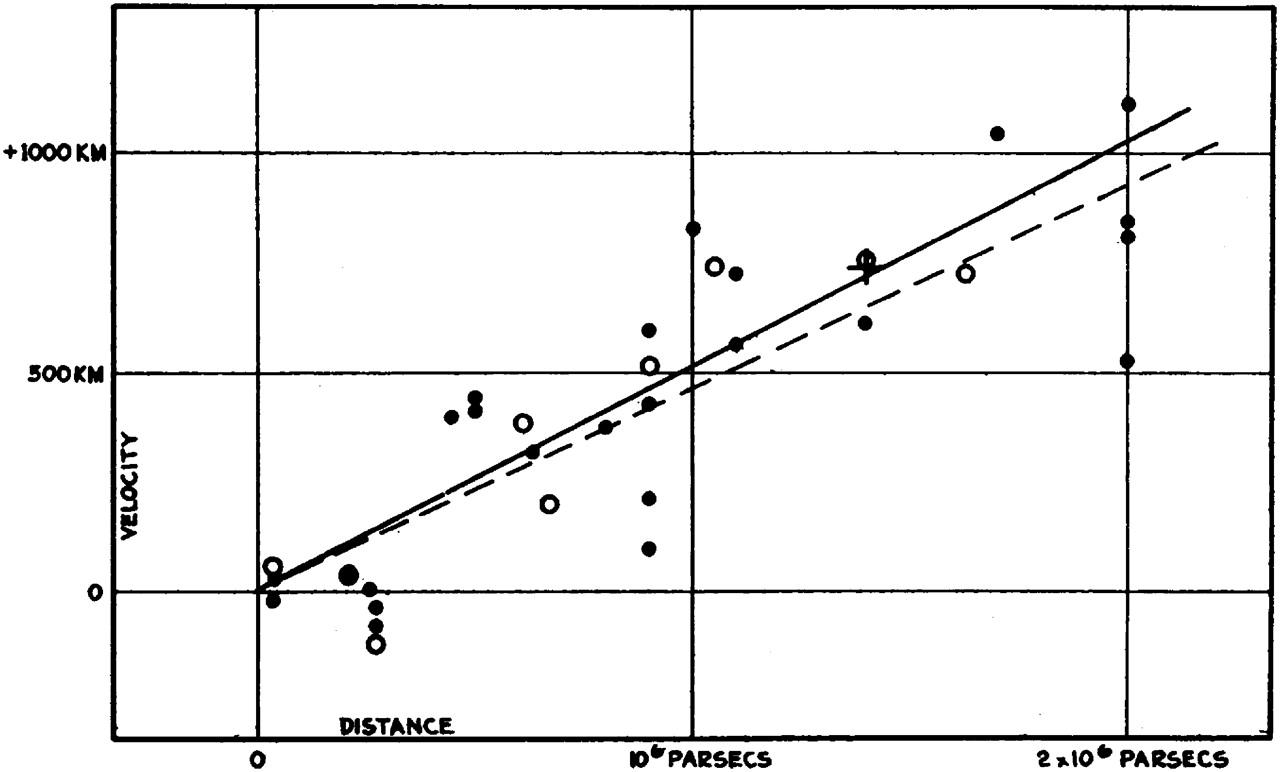
\includegraphics[height=4cm]{F2.large.jpg}
  \end{block}
  \begin{block}{}
    \mentiinvitation{}
    \begin{enumerate}
      \item{70 km per second per megaparsec}
      \item{100 km per second per megaparsec}
      \item{\correctanswer{500 km per second per megaparsec}}
    \end{enumerate}
  \end{block}
\end{frame}


\begin{frame}{Falling estimates of $H_0$ 1920 - 1980}
    \imageandcredit{Trimble_HistoryOfHubbleConstant.png}{height=7cm}{Trimble}{1.5}{-2.3}
\end{frame}


\begin{frame}{Distances had been underestimated}
   Several revisions (distance up, $H_0$ down) followed:
    \begin{enumerate}
      \item{Two types of Cepheids}
      \item{Interstellar absorption of light}
      \itemandimageandcredit{Scott effect (visible galaxies tend to be brighter than average)}{Scott_Elizabeth.jpeg}{height=3cm}{MacTutor}{-4}{-1.3}
      \item{Regions of hot gas were being misidentified as bright stars}
    \end{enumerate}
\end{frame}


\begin{frame}{Hubble Space Telescope}
  \begin{itemize}
  \item{The Hubble Space Telescope was built (in part) to measure $H_0$.}
  \itemandimageandcredit{Lead investigator Wendy Freedman.}{Wendy_Freedman_4617812603.jpg}{height=2.5cm}{pollosaurio}{-4}{-1.3}
  \item{Used supernovae as additional standard candles.}
  \item{$H_0 = 72 \pm 8$ kilometers per second per megaparsec.}
  \end{itemize}
\end{frame}


\begin{frame}{More recent values - diverging opinion}
  \imageandcredit{Freedman_RecentHistoryOfH0.png}{height=5cm}{W. Freedman}{1}{-1}
  \begin{itemize}
  \item{Blue results use standard candles: $H_0 = 74 \pm 1.4$ kilometers per second per megaparsec.}
  \item{Red results use data from the early Universe: $67.4 \pm 0.6$ kilometers per second per megaparsec.}
  \end{itemize}
\end{frame}


\begin{frame}{$H_0$ from early Universe data}
  \begin{itemize}
  \item{For 400,000 years after the Big Bang, the Universe was opaque. Then it became transparent, and we can today observe (red-shifted) light from then (the \textit{Cosmic Microwave Background)}.}
  \item{The distance that light could travel in those first 400,000 years can be seen statistically in these observations. Trigonometry then gives us the distance from which we are viewing that light.}
  \item{Redshift is easy - the spectrum has a prominent peak.}
  \item{Finally, correct for the evolution of $H_0$ from then to now.}
  \end{itemize}
\end{frame}


\begin{frame}{Hubble tension}
  \imageandcredit{Freedman_RecentHistoryOfH0.png}{height=5.5cm}{W. Freedman}{0.75}{-1.5}
  Should we be worried by the discrepancy? It could indicate that our theory is wrong. But it might also just be a systematic error in one of the measurements.
\end{frame}


\begin{frame}{Hubble constant - past and future}
  \begin{itemize}
  \itemandimageandcredit{$H_0$ isn't constant over cosmic timescales. The evolution is controlled by the contents of the Universe.}{h0.png}{height=5cm}{LW}{-2}{1.7}
  \item{Matter - mostly dark matter, but also hydrogen and helium - tends to push $H_0$ towards zero (no expansion).}
  \item{But the Universe also contains dark energy, and this opposes this trend. In the distant future the expansion will stabilise near 57 kilometers per second per megaparsec.}
  \end{itemize}
\end{frame}


%%%%%%%%%%%%%%% Start of end material %%%%%%%%%%%%%%%



\begin{frame}{Where to find this document}
  \begin{block}{}
  \begin{itemize}
  \item{You can find the presentation at \alert{\url{https://tinyurl.com/bycke8v6}}}
  \end{itemize}
  \end{block}
\end{frame}


\begin{frame}{Image credits}
  \begin{enumerate}
  \tiny {
  \item{Hubble Deep Field: Source: NASA. From \url{https://en.wikipedia.org/wiki/File:Hubble_ultra_deep_field_high_rez_edit1.jpg}}
  \item{M31: Source: David Dayag. Licensed under the Creative Commons Attribution-Share Alike 4.0 International license \url{https://creativecommons.org/licenses/by-sa/4.0/deed.en}. From \url{https://upload.wikimedia.org/wikipedia/commons/thumb/8/8c/Andromeda_Galaxy_560mm_FL.jpg/1024px-Andromeda_Galaxy_560mm_FL.jpg}.}
  \item{Poe: Source: Public domain. From \url{https://en.wikipedia.org/wiki/Edgar_Allan_Poe\#/media/File:Edgar_Allan_Poe,_circa_1849,_restored,_squared_off.jpg}}
  \item{Hubble: Source: Public domain (by Johan Hagemeyer (1884-1962)). From \url{https://commons.wikimedia.org/wiki/File:Studio_portrait_photograph_of_Edwin_Powell_Hubble.JPG}}
  \item{Einstein: Source: Public domain. From \url{https://upload.wikimedia.org/wikipedia/commons/thumb/c/c3/08608_einstein_1916.jpg/512px-08608_einstein_1916.jpg}}
  \item{Curved spacetime: Source: Mysid. Licensed under the Creative Commons Attribution-Share Alike 3.0 Unported license \url{https://creativecommons.org/licenses/by-sa/3.0/deed.en}. From \url{https://commons.wikimedia.org/wiki/File:Spacetime_lattice_analogy.svg}}
  \item{Friedmann: Source: Public domain. From \url{https://upload.wikimedia.org/wikipedia/commons/6/62/Aleksandr_Fridman.png}}
  \item{Lemaiitre: Source: Public domain. From \url{https://upload.wikimedia.org/wikipedia/commons/thumb/5/51/Georges_Lema\%C3\%AEtre_1930s.jpg/512px-Georges_Lema\%C3\%AEtre_1930s.jpg}}  
  \item{Redshift: Source: Georg Wiora. Licensed under the Creative Commons Attribution-Share Alike 2.5 Generic license \url{https://creativecommons.org/licenses/by-sa/2.5/deed.en}. From \url{https://commons.wikimedia.org/wiki/File:Redshift.svg}}
  \item{Slipher: Source: Lowell Archive. Licensed under the Creative Commons Attribution-Share Alike 4.0 International license \url{https://creativecommons.org/licenses/by-sa/4.0/deed.en}. From \url{https://upload.wikimedia.org/wikipedia/commons/a/a7/V.M._Slipher.gif}, converted to png}  
  } % end tiny
  \end{enumerate}
\end{frame}

\begin{frame}{Image credits}
  \begin{enumerate}\addtocounter{enumi}{10}
  \tiny {
  \item{Leavitt: Source: Public domain. From \url{https://upload.wikimedia.org/wikipedia/commons/thumb/3/3b/Leavitt_aavso.jpg/256px-Leavitt_aavso.jpg}}
  \item{Millikan, Lamaitre, Einstein: Source: Public domain. From \url{https://upload.wikimedia.org/wikipedia/commons/c/c6/MillikanLemaitreEinstein.jpg}}
  \item{Hubble at Mt Wilson: Source: Edwin Hubble Papers/Courtesy of Huntington Library, San Marino, Calif. From \url{https://www.npr.org/2015/04/25/401843663/hubbles-other-telescope-and-the-day-it-rocked-our-world?t=1636381997027}}
  \item{Hubble plot: Source: Hubble, H., ``A relation between distance and radial velocity among extra-galactic nebulae'', PNAS March 15, 1929 15 (3) 168-173. From \url{https://www.pnas.org/content/15/3/168/tab-figures-data}}
  \item{Trimble plot: Source: Trimble, V., ``H0: The incredible shrinking constant'', 1925-1975. 1996 PASP 108 1073. From \url{https://iopscience.iop.org/article/10.1086/133837/meta}}
  \item{Scott: Source: Public domain. From \url{https://mathshistory.st-andrews.ac.uk/Biographies/Scott_Elizabeth/Scott_Elizabeth.jpeg}}
  \item{Freedman: Source: pollosaurio. Licensed under the Creative Commons Attribution 2.0 Generic license \url{https://creativecommons.org/licenses/by/2.0/}. From \url{https://commons.wikimedia.org/wiki/File:Wendy_Freedman_(4617812603).jpg}}
  \item{Freedman plot: Source: Friedmann, W. L. "Cosmology at a Crossroads: Tension with the Hubble Constant." Nature Astronomy 1 (2017): 0169. From \url{https://arxiv.org/abs/1706.02739}}
  \item{H0 History plot: Source: Original work. From \url{https://github.com/LorneWhiteway/HistoryOfH0Talk/blob/master/h0.png}}
  } % end tiny
  \end{enumerate}
\end{frame}



\end{document}
